\subsubsubsection{Odabir plana ishrane}

\begin{itemize}
    \item Kratak opis:
        \begin{itemize}
            \item Registrovani klijent bira svoj plan ishrane.
        \end{itemize}
    \item Učesnici:
        \begin{itemize}
            \item Registrovan klijent
        \end{itemize}
    \item Preduslovi:
        \begin{itemize}
            \item Klijent mora biti registrovan i ulogovan na aplikaciju.
            \item Klijent nema odabran plan ishrane.
        \end{itemize}
    \item Postuslovi:
        \begin{itemize}
            \item Podaci su uspešno sačuvani u bazi podataka, zakazana je dostava hrane i skinut je novac sa računa za prvu nedelju.
        \end{itemize}
    \item Osnovni tok:
        \begin{enumerate}
            \item Sistem prikazuje klijentu formu za odabir plana.
            \item Klijent bira svoje preference za tip obroka za koji želi da dobija recepte.
            \item Klijent bira za koliko osoba će biti obrok.
            \item Klijent bira koliko obroka u nedelji želi.
            \item Sistem prikazuje klijentu cenu odabranog plana.
            \item Klijent potvrđuje odabir plana.
            \item Sistem prikazuje klijentu formu za unos adrese, željenog dana dostave i satnice dostave.
            \item Klijent potvđuje podatke koje je uneo.
            \item Sistem prikazuje klijentu recepte koje može odabrati.
            \item Klijent bira recepte.
            \item Sistem prikazuje klijentu formu za unos detalja o plaćanju.
            \item Klijent potvrđuje svoje podatke o plaćanju i potvrđuje narudžbinu.
            \item Sistem čuva podatke i skida novac sa klijentovog računa.
            \item Sistem prikazuje poruku o uspešnosti. 
        \end{enumerate}
    \item Alternativni tok:
        \begin{itemize}
            \item Ukoliko klijent odustane od odabira u bilo kom trenutku, pri narednom logovanju može da nastavi od poslednjeg potvrđenog odabira.
            \item[13.a] Ukoliko sistem ne uspe da obavi skidanje novca sa računa, obaveštava klijenta o tome sa porukom o grešci. Proces se nastavlja u 11. koraku osnovnog toka.
        \end{itemize}
    \item Dodatne informacije:
        \begin{itemize}
            \item Preference za tip obroka su: obroci zasnovani na mesu i povrću, obroci zasnovani na povrću, obroci namenjeni korišćenju od strane porodice, obroci kod kojih se pazi na broj kalorija, brzi i jednostavni obroci i obroci zasnovani na pesketarijanskoj ishrani. 
            \item Obrok može biti za 2 ili 4 osobe.
            \item Moguće je odbrati od 2 do 6 obroka u nedelji.
        \end{itemize}
\end{itemize}

\begin{figure}[H]
\begin{center}
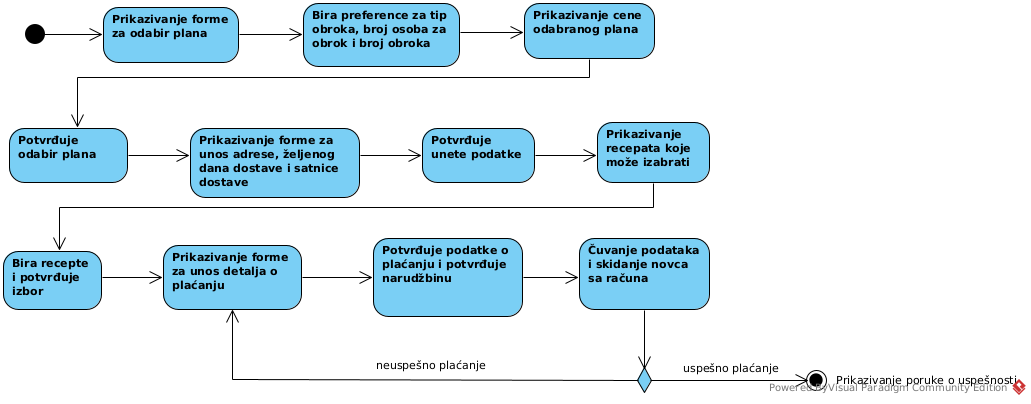
\includegraphics[width=\textwidth]{activity_select_meal_plan.png}
\end{center}
    \caption{Dijagram aktivnosti odabira plana ishrane}
\label{fig:ActivitySelectMealPlan}
\end{figure}
